\chapter{El mecanismo de Higgs: cómo adquiere masa un bosón gauge}

Ahora reunimos las dos ideas desarrolladas en la clase anterior. Un campo escalar complejo con una simetría global \(U(1)\) rota contiene una oscilación radial masiva y una oscilación angular sin masa. Una teoría localmente invariante bajo \(U(1)\) contiene un campo gauge sin masa. Cuando el escalar está cargado y su magnitud de equilibrio es distinta de cero, estas afirmaciones no pueden simplemente combinarse. El modo angular y el campo gauge se combinan: el campo gauge adquiere masa, el bosón de Goldstone aparente deja de ser una partícula independiente y permanece el modo radial de Higgs.

Tomaremos el fotón como modelo de bosón gauge, pero no como conclusión física. La simetría electromagnética \(U(1)\) no está rota en el vacío, así que el fotón real no tiene masa. El mismo mecanismo actúa sobre \(W^\pm\) y \(Z\) en la teoría electrodébil, donde el grupo gauge y el multiplete escalar son más complicados. El modelo abeliano permite ver el mecanismo sin ocultarlo bajo la teoría de grupos.

\begin{classroomqa}
\audiencequestion{¿La explicación anterior quería decir que el mecanismo de Higgs da masa al fotón real?\lecturetimestamp{00:00:23}}
\lecturerresponse{No. Preguntamos qué ocurriría \emph{si} el \(U(1)\) asociado al fotón estuviera en una fase rota. Ese fotón hipotético adquiriría masa. El vacío electromagnético real no está en esa fase; en física de partículas, la aplicación del mecanismo es, en cambio, la masa de \(W\) y \(Z\).}
\end{classroomqa}

La simetría asociada a la conservación de la carga eléctrica es la rotación de fase
\begin{equation}
  \phi(x)\longmapsto e^{i\theta}\phi(x),
\end{equation}
una rotación interna llamada \(U(1)\). Un superconductor proporciona una analogía real de la fase rota. En su interior, el campo electromagnético tiene una profundidad de penetración finita y, en aspectos importantes, se comporta como un campo masivo. En el exterior reaparece el fotón ordinario sin masa.

\section{Qué significa la masa para un campo}

\subsection{Dispersión y brecha en el momento nulo}

Conviene precisar qué entendemos por masa antes de introducir el campo de Higgs. Para una onda,
\begin{equation}
  E=\hbar\omega,
  \qquad
  p=\hbar k,
  \label{eq:l08-quantum-wave}
\end{equation}
así que las gráficas \((E,p)\) y \((\omega,k)\) contienen la misma información, salvo por factores de \(\hbar\). En el espacio vacío, una excitación relativista sin masa satisface
\begin{equation}
  E=c|p|,
  \qquad
  \omega=c|k|.
  \label{eq:l08-massless-dispersion}
\end{equation}
Los dos signos de \(k\) distinguen sentidos de propagación opuestos. Lo esencial es que \(\omega\) tiende a cero cuando lo hace \(k\).

Una partícula relativista masiva satisface
\begin{equation}
  E^2=c^2p^2+m^2c^4.
  \label{eq:l08-massive-dispersion}
\end{equation}
En unidades \(c=\hbar=1\),
\begin{equation}
  \omega^2=k^2+m^2.
\end{equation}
En \(k=0\), la energía es \(E=mc^2\), o simplemente \(m\) en unidades naturales. Por tanto, la masa es la brecha de energía distinta de cero del modo con momento nulo.

\begin{figure}[htbp]
\centering
\begin{adjustbox}{max width=\linewidth}
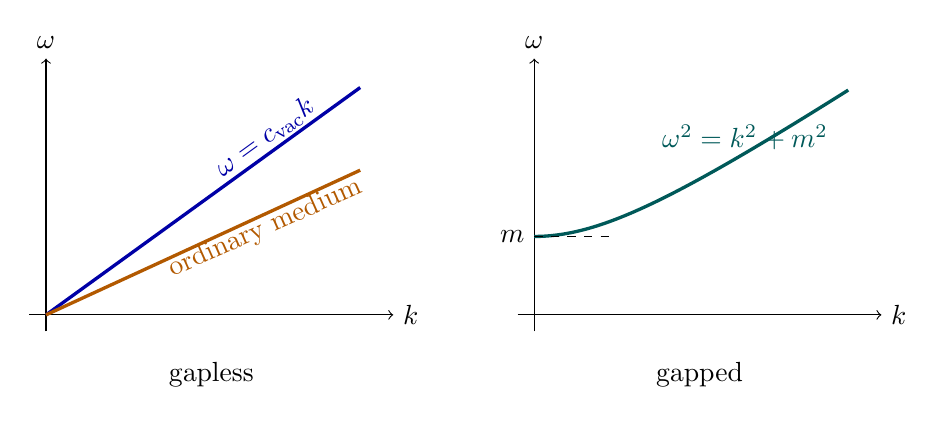
\begin{tikzpicture}[x=1.05cm,y=1.05cm]
  \begin{scope}
    \draw[->] (-0.2,0) -- (4.2,0) node[right] {\(k\)};
    \draw[->] (0,-0.2) -- (0,3.1) node[above] {\(\omega\)};
    \draw[very thick,blue!65!black] (0,0) -- (3.8,2.75);
    \draw[very thick,orange!70!black] (0,0) -- (3.8,1.75);
    \node[blue!65!black,rotate=36] at (2.65,2.15)
      {\(\omega=c_{\rm vac}k\)};
    \node[orange!70!black,rotate=24] at (2.65,1.05)
      {ordinary medium};
    \node[below] at (2,-0.45) {gapless};
  \end{scope}
  \begin{scope}[xshift=6.2cm]
    \draw[->] (-0.2,0) -- (4.2,0) node[right] {\(k\)};
    \draw[->] (0,-0.2) -- (0,3.1) node[above] {\(\omega\)};
    \draw[very thick,domain=0:3.8,samples=120,smooth,teal!70!black]
      plot (\x,{sqrt(0.9+0.45*\x*\x)});
    \draw[dashed] (0,0.95) -- (1.0,0.95);
    \node[left] at (0,0.95) {\(m\)};
    \node[teal!70!black] at (2.55,2.15)
      {\(\omega^2=k^2+m^2\)};
    \node[below] at (2,-0.45) {gapped};
  \end{scope}
\end{tikzpicture}
\end{adjustbox}
\caption{Cambiar la velocidad de propagación modifica la pendiente de una relación de dispersión sin brecha. Dar masa a la excitación abre una brecha distinta de cero en \(k=0\).}
\label{fig:l08-dispersion}
\end{figure}

Un material transparente ordinario puede reducir la velocidad de fase de una onda sin crear esta brecha de masa relativista. En una interfaz, la frecuencia incidente se mantiene fija, mientras que el número de onda se ajusta a la relación de dispersión del medio. Cambiar la pendiente no equivale a elevar la ordenada al origen.
\editorialnote{Un material puede tener varias ramas electromagnéticas, y un plasma o un medio resonante puede presentar una brecha distinta de cero asociada a la frecuencia de plasma. La comparación de esta clase se refiere específicamente a una rama refractiva ordinaria y a la respuesta superconductora. En términos más generales, que no haya brecha significa que \(\omega(k)\to0\) cuando \(k\to0\); no se requiere una relación lineal exacta en todos los medios no relativistas.}

\begin{classroomqa}
\audiencequestion{¿Adquiere masa un fotón cada vez que atraviesa la materia, por ejemplo, un prisma?\lecturetimestamp{00:03:02}}
\lecturerresponse{No. La refracción puede cambiar la relación entre la frecuencia y el número de onda y, por tanto, la velocidad de propagación, aunque la rama siga pasando por \(\omega=0\) en \(k=0\). En cambio, una fase superconductora confiere a la respuesta electromagnética una longitud inversa de penetración finita, análoga a una masa.}
\end{classroomqa}

\begin{classroomqa}
\audiencequestion{Cuando la luz de frecuencia fija entra en el vidrio, ¿cambia el número de onda?\lecturetimestamp{00:09:20}}
\lecturerresponse{Sí. La invariancia ante traslaciones temporales en una interfaz estacionaria mantiene fija la frecuencia. Como la curva de dispersión tiene una pendiente distinta en el vidrio, el mismo \(\omega\) corresponde a un \(k\) distinto y, por tanto, a una longitud de onda diferente.}
\end{classroomqa}

La pendiente
\begin{equation}
  v_g=\frac{d\omega}{dk}
\end{equation}
es la velocidad de grupo de un paquete de ondas. Si esa pendiente varía con \(k\), las distintas componentes de Fourier se desplazan a velocidades diferentes y el paquete se dispersa. Por eso la relación \(\omega(k)\) se llama relación de \emph{dispersión}.

\begin{classroomqa}
\audiencequestion{¿Cómo se llama la curva y qué representa su pendiente?\lecturetimestamp{00:11:02}}
\lecturerresponse{La curva es la relación de dispersión. Su derivada \(d\omega/dk\) es la velocidad de grupo. Una pendiente constante da la misma velocidad a todas las longitudes de onda; si la pendiente varía, el paquete de ondas se ensancha. Para lo que nos ocupa, la distinción decisiva es si la curva alcanza el origen o tiene una brecha.}
\end{classroomqa}

\subsection{Una oscilación homogénea es una partícula en reposo}

El modo \(k=0\) tiene longitud de onda infinita: el campo está desplazado en la misma cantidad en todas partes. Liberemos un desplazamiento homogéneo. Si el campo oscila con una frecuencia distinta de cero, el cuanto correspondiente tiene energía en reposo distinta de cero y es masivo. Si en esa dirección no hay fuerza restauradora, la frecuencia se anula y el modo no tiene masa.

Esta afirmación es clásica. No requiere que partículas separadas espacialmente estén en una superposición cuántica. Una configuración clásica homogénea del campo consiste simplemente en un mismo valor del campo repetido por todo el espacio.

\begin{classroomqa}
\audiencequestion{Si se desplaza todo un campo a la vez, ¿es eso lo mismo que el entrelazamiento cuántico?\lecturetimestamp{00:10:04}}
\lecturerresponse{No. Un campo clásico homogéneo es una sola configuración clásica. El entrelazamiento correlaciona alternativas cuánticas distintas, como las configuraciones de espín arriba--abajo y abajo--arriba. Preparar el mismo valor del campo en muchos puntos no constituye por sí solo entrelazamiento, ni implica una respuesta causal instantánea.}
\end{classroomqa}

Para un campo real con normalización canónica,
\begin{equation}
  \mathcal L
  =\frac12\partial_\mu\varphi\,\partial^\mu\varphi-V(\varphi),
\end{equation}
desarrollemos alrededor de un equilibrio \(\varphi_0\):
\begin{equation}
  V(\varphi_0+\eta)
  =V(\varphi_0)
   +\frac12V''(\varphi_0)\eta^2+\cdots.
\end{equation}
El término lineal se anula en el mínimo, y la ecuación de campo da
\begin{equation}
  \omega^2=\bm{k}^2+m^2,
  \qquad
  m^2=V''(\varphi_0).
  \label{eq:l08-curvature-mass}
\end{equation}
Por tanto, la masa es la curvatura del potencial en la dirección del movimiento. Una dirección plana tiene curvatura nula y da lugar a un modo sin masa.

\section{El escalar complejo roto}

\subsection{Movimiento radial y angular}

Escribamos un escalar complejo en coordenadas cartesianas y polares:
\begin{equation}
  \phi=\phi_R+i\phi_I=\rho e^{i\alpha},
  \qquad
  \phi^*=\phi_R-i\phi_I=\rho e^{-i\alpha}.
  \label{eq:l08-polar-field}
\end{equation}
El plano complejo es un espacio de campos \emph{interno}. En cada punto físico del espacio-tiempo \(x\), el par
\((\phi_R(x),\phi_I(x))\) especifica un punto de ese plano interno.
Ninguno de los ejes internos indica una dirección en el laboratorio.

\begin{figure}[htbp]
\centering
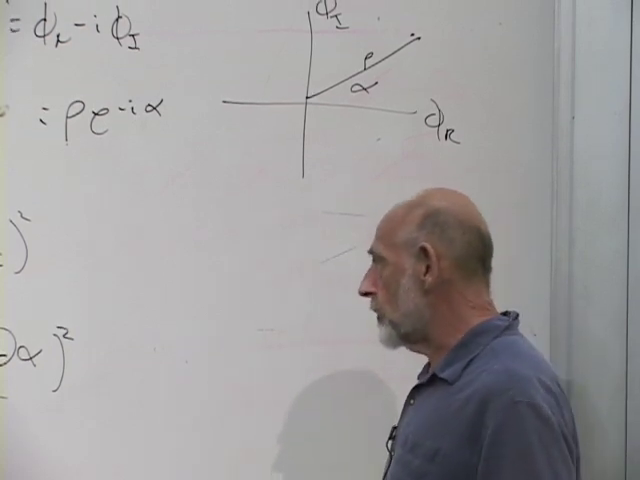
\includegraphics[width=0.72\textwidth]{lecture_08_figure_02.png}
\caption{El escalar complejo representado en su plano interno \((\phi_R,\phi_I)\). El radio es \(\rho\) y \(\alpha\) es la fase interna.}
\lectureframe{00:24:41}
\label{fig:l08-internal-plane}
\end{figure}

El término cinético del escalar se convierte en
\begin{align}
  \partial_\mu\phi^*\,\partial^\mu\phi
  &=
  \partial_\mu\phi_R\,\partial^\mu\phi_R
  +\partial_\mu\phi_I\,\partial^\mu\phi_I
  \notag\\
  &=
  \partial_\mu\rho\,\partial^\mu\rho
  +\rho^2\partial_\mu\alpha\,\partial^\mu\alpha.
  \label{eq:l08-polar-kinetic}
\end{align}
Un potencial invariante bajo \(U(1)\) global depende de \(\phi^*\phi=\rho^2\), no de \(\alpha\). Por ejemplo,
\begin{equation}
  V(\phi)
  =\lambda\left(\phi^*\phi-\frac{f^2}{2}\right)^2,
  \qquad \lambda>0.
  \label{eq:l08-mexican-hat}
\end{equation}
Sus mínimos forman un círculo. La ley es invariante bajo una rotación común de fase, pero elegir una fase de equilibrio selecciona un punto del círculo.

\begin{figure}[htbp]
\centering
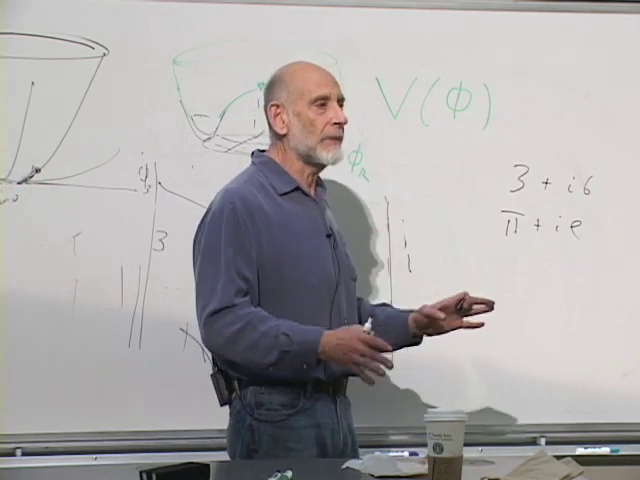
\includegraphics[width=0.78\textwidth]{lecture_08_figure_03.png}
\caption{Esquema del potencial radial dibujado en la pizarra. El potencial es simétrico bajo rotaciones del valor interno del campo, aunque el propio campo no tenga por qué estar en el origen.}
\lectureframe{00:34:22}
\label{fig:l08-radial-potential-board}
\end{figure}

\begin{figure}[htbp]
\centering
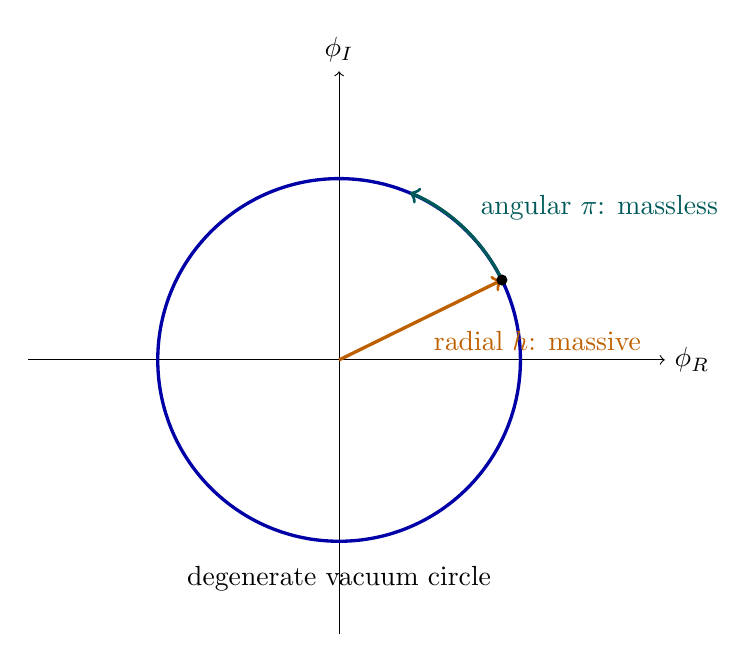
\begin{tikzpicture}[x=0.94cm,y=0.94cm]
  \draw[->] (-4.2,0) -- (4.4,0) node[right] {\(\phi_R\)};
  \draw[->] (0,-3.7) -- (0,3.9) node[above] {\(\phi_I\)};
  \draw[very thick,blue!65!black] (0,0) circle (2.45);
  \draw[->,very thick,orange!75!black] (0,0) -- (2.2,1.08);
  \draw[->,very thick,teal!70!black]
    (2.2,1.08) arc[start angle=26,end angle=67,radius=2.45];
  \node[orange!75!black,below right] at (1.15,0.52)
    {radial \(h\): massive};
  \node[teal!70!black,above right] at (1.78,1.76)
    {angular \(\pi\): massless};
  \fill (2.2,1.08) circle (2pt);
  \node[below] at (0,-2.65) {degenerate vacuum circle};
\end{tikzpicture}
\caption{La teoría global rota tiene curvatura normal al círculo de vacíos, pero no a lo largo de este. El modo radial de Higgs es masivo; el modo angular de Goldstone no tiene masa.}
\label{fig:l08-radial-angular}
\end{figure}

Definamos
\begin{equation}
  \phi(x)=\frac{f+h(x)}{\sqrt2}
           e^{i\pi(x)/f}.
  \label{eq:l08-canonical-polar}
\end{equation}
Cerca del vacío seleccionado, \(h\) mide el desplazamiento radial y \(\pi\) mide el desplazamiento tangencial, ambos con dimensiones canónicas. Al sustituir en la ec.~\eqref{eq:l08-polar-kinetic} se obtiene
\begin{equation}
  \partial_\mu\phi^*\,\partial^\mu\phi
  =
  \frac12(\partial_\mu h)^2
  +\frac12\left(1+\frac{h}{f}\right)^2
            (\partial_\mu\pi)^2.
  \label{eq:l08-global-expanded}
\end{equation}
El potencial de la ec.~\eqref{eq:l08-mexican-hat} aporta
\begin{equation}
  m_h^2=2\lambda f^2,
  \qquad
  m_\pi^2=0.
  \label{eq:l08-global-masses}
\end{equation}
A energías muy inferiores a \(m_h\), el movimiento radial resulta costoso, así que podemos fijar temporalmente \(h=0\). El lagrangiano restante contiene solo \(\frac12(\partial\pi)^2\), sin término \(\pi^2\). Este es el bosón de Goldstone.\editorialnote{En dos momentos, la explicación oral invierte los nombres y dice que, al engullir el Goldstone, el bosón de Higgs adquiere masa. El cálculo de la pizarra y el resto de la clase establecen el resultado pretendido: la curvatura radial ya confiere masa al modo de Higgs, mientras que el bosón gauge adquiere el modo de Goldstone y se vuelve masivo.}

\begin{classroomqa}
\audiencequestion{¿Es esta la única ruptura espontánea de simetría en el modelo estándar?\lecturetimestamp{00:16:39}}
\lecturerresponse{La fase de Higgs electrodébil es el mecanismo de ruptura de simetría establecido que nos interesa aquí. La simetría real es \(SU(2)_L\times U(1)_Y\), no este único \(U(1)\), y la QCD tiene otras estructuras del vacío, como la ruptura de la simetría quiral. El ejemplo abeliano es un modelo deliberadamente reducido del mecanismo de adquisición de masa de los bosones gauge.}
\end{classroomqa}

\begin{classroomqa}
\audiencequestion{¿El Higgs da masa a todas las partículas, incluida él mismo?\lecturetimestamp{00:17:11}}
\lecturerresponse{Hay que distinguir entre un sí y un no. La simetría electrodébil prohíbe masas desnudas para \(W\), \(Z\) y los fermiones del modelo estándar; sus masas aparecen cuando el campo de Higgs adquiere una magnitud de equilibrio distinta de cero. La masa radial del Higgs proviene de la curvatura de su propio potencial. Otras partículas hipotéticas pueden tener masas permitidas por la simetría y ajenas a este mecanismo.}
\end{classroomqa}

La clase relaciona esas masas permitidas por la simetría con partículas potencialmente muy pesadas y difíciles de observar, y menciona la materia oscura como posible ejemplo. Se trata de una motivación, no de una predicción de masa.
\editorialnote{La escala de masa de la materia oscura sigue siendo desconocida. La sugerencia de la clase de que podría tratarse de una partícula con una masa de alrededor de mil veces la masa del protón es una especulación histórica, no una propiedad de la materia oscura establecida experimentalmente.}

\begin{classroomqa}
\audiencequestion{¿\(\rho\) es un radio físico o el valor del campo? ¿Qué es exactamente lo que tiene simetría radial?\lecturetimestamp{00:33:08}}
\lecturerresponse{En cada punto del espacio-tiempo, el valor del campo es un punto de un plano complejo auxiliar, y \(\rho=|\phi|\) es la distancia de ese punto al origen. El \emph{potencial} tiene simetría radial en este plano interno: todos los puntos con el mismo \(\rho\) tienen la misma energía potencial. Este radio no es una distancia en el espacio ordinario.}
\end{classroomqa}

\begin{classroomqa}
\audiencequestion{¿Podría una perturbación radial lo bastante violenta llevar el campo por encima del máximo central hasta el otro lado del potencial?
\lecturetimestamp{00:36:00}}
\lecturerresponse{En principio, una configuración local con suficiente energía puede superar la barrera. Desplazar por encima de ella un campo macroscópico homogéneo requeriría una energía enorme, y una perturbación violenta genérica disiparía energía en muchos modos del campo en lugar de llegar coherentemente al punto opuesto. La aproximación de baja energía fija \(\rho\) precisamente porque en ese régimen no son accesibles excursiones radiales de ese tipo.}
\end{classroomqa}

\section{Por qué el plano complejo no es el espacio-tiempo}

La distinción entre coordenadas físicas e internas merece que nos detengamos en ella como en la clase. Un campo se llama escalar porque es invariante bajo rotaciones de los ejes de coordenadas físicas. Dos campos escalares reales \(\phi_R(x)\) y \(\phi_I(x)\) siguen siendo dos escalares bajo esas rotaciones. Podemos agruparlos en un solo número complejo, pero esta notación no los convierte en componentes de un vector espacial.

Una transformación global \(U(1)\) rota los \emph{valores} del campo:
\begin{equation}
\begin{aligned}
  \phi(x)&\longmapsto e^{i\theta}\phi(x),
  \\
  \rho(x)&\longmapsto\rho(x),
  \\
  \alpha(x)&\longmapsto\alpha(x)+\theta.
\end{aligned}
  \label{eq:l08-global-shift}
\end{equation}
Se usa la misma constante \(\theta\) en todos los puntos del espacio-tiempo. En consecuencia, \(\partial_\mu\alpha\) no cambia. Esta es una simetría tanto del potencial como del término cinético ordinario. Si se permite que \(\theta\) dependa de \(x\), la derivada detecta esa variación y el argumento cambia.

\section{Hacer local la rotación de fase}

\subsection{La derivada ordinaria deja de funcionar}

Sea
\begin{equation}
  \phi'(x)=e^{i\theta(x)}\phi(x).
  \label{eq:l08-local-phase}
\end{equation}
Entonces
\begin{equation}
  \partial_\mu\phi'
  =e^{i\theta}
    \left(\partial_\mu\phi+i\,\partial_\mu\theta\,\phi\right).
  \label{eq:l08-ordinary-derivative-fails}
\end{equation}
El término adicional proporcional a \(\partial_\mu\theta\) impide que \(\partial_\mu\phi\) se transforme como \(\phi\). Por tanto, \(\partial_\mu\phi^*\partial^\mu\phi\) no es invariante bajo rotaciones de fase locales arbitrarias.

\begin{figure}[htbp]
\centering
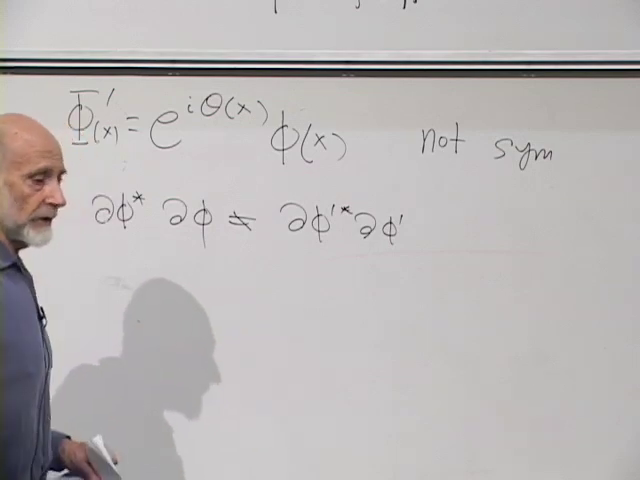
\includegraphics[width=0.78\textwidth]{lecture_08_figure_04.png}
\caption{La pizarra recoge la transformación local de fase y muestra que el término con la derivada ordinaria no conserva la invariancia.}
\lectureframe{00:46:49}
\label{fig:l08-local-not-symmetry}
\end{figure}

Introduzcamos un potencial vector y fijemos una convención para usarla coherentemente:
\begin{equation}
  D_\mu=\partial_\mu+i g A_\mu,
  \qquad
  A_\mu'=A_\mu-\frac1g\partial_\mu\theta.
  \label{eq:l08-covariant-convention}
\end{equation}
Ahora,
\begin{align}
  D_\mu'\phi'
  &=
  \left(\partial_\mu+i g A_\mu'\right)
  e^{i\theta}\phi
  \notag\\
  &=
  e^{i\theta}
  \left[
    \partial_\mu\phi+i(\partial_\mu\theta)\phi
    +i g A_\mu\phi-i(\partial_\mu\theta)\phi
  \right]
  \notag\\
  &=e^{i\theta}D_\mu\phi.
  \label{eq:l08-covariant-transform}
\end{align}
Los términos no deseados se cancelan. La derivada conjugada es
\begin{equation}
  (D_\mu\phi)^*
  =(\partial_\mu-i g A_\mu)\phi^*,
\end{equation}
y su fase opuesta se cancela en el producto
\begin{equation}
  (D_\mu\phi)^*D^\mu\phi.
\end{equation}

\begin{classroomqa}
\audiencequestion{¿En la clase anterior se escribió con el signo opuesto la transformación del campo gauge?\lecturetimestamp{00:48:04}}
\lecturerresponse{Invertir simultáneamente el signo en \(D_\mu\) y en la ley de transformación es solo una convención. Con \(D_\mu=\partial_\mu+i gA_\mu\) y \(\phi'=e^{i\theta}\phi\), la coherencia exige \(A_\mu'=A_\mu-g^{-1}\partial_\mu\theta\). La convención alternativa funciona igual de bien si se cambian todos los signos a la vez.}
\end{classroomqa}

\begin{classroomqa}
\audiencequestion{¿El uso de una forma mayúscula o minúscula de \(\phi\) en la pizarra indica un campo distinto?\lecturetimestamp{00:55:02}}
\lecturerresponse{No se pretende indicar ninguna diferencia. La variación en la forma de la letra se debe a la caligrafía; no indica una operación adicional ni un segundo escalar. Las distinciones con significado son la prima, el asterisco de conjugación compleja y el índice espacio-temporal.}
\end{classroomqa}

\begin{classroomqa}
\audiencequestion{¿Es la conjugación compleja la misma operación que subir o bajar el índice de Lorentz en el término cinético?
\lecturetimestamp{00:56:50}}
\lecturerresponse{No. El asterisco conjuga el campo complejo interno. Los índices de Lorentz se suben con la métrica del espacio-tiempo:
\(D^\mu=g^{\mu\nu}D_\nu\). Un escalar de Lorentz requiere la contracción \((D_\mu\phi)^*D^\mu\phi\); ambas operaciones aparecen y cumplen funciones distintas.}
\end{classroomqa}

\subsection{El campo gauge tiene su propia dinámica}

El tensor de campo
\begin{equation}
  F_{\mu\nu}=\partial_\mu A_\nu-\partial_\nu A_\mu
  \label{eq:l08-field-strength}
\end{equation}
es invariante gauge porque se cancelan las dos derivadas segundas mixtas de \(\theta\). Sus componentes temporales--espaciales contienen el campo eléctrico, y sus componentes espaciales--espaciales contienen el campo magnético. Por tanto, la electrodinámica escalar queda descrita por
\begin{equation}
  \mathcal L
  =(D_\mu\phi)^*D^\mu\phi
  -V(\phi^*\phi)
  -\frac14F_{\mu\nu}F^{\mu\nu}.
  \label{eq:l08-abelian-higgs}
\end{equation}
El campo cargado que aparece aquí es bosónico. No es el campo del electrón, que es un fermión. Un núcleo de helio cargado o un condensado de pares de Cooper ilustran cómo puede surgir un grado de libertad bosónico cargado.

Antes de la ruptura de simetría, el término gauge contiene derivadas de \(A_\mu\), pero ningún término de masa directo. Podríamos intentar añadir
\begin{equation}
  \frac12m_A^2A_\mu A^\mu,
\end{equation}
pero, bajo la ec.~\eqref{eq:l08-covariant-convention},
\begin{equation}
  A_\mu A^\mu
  \longmapsto
  \left(A_\mu-\frac1g\partial_\mu\theta\right)
  \left(A^\mu-\frac1g\partial^\mu\theta\right),
  \label{eq:l08-bare-mass-fails}
\end{equation}
que no es igual a \(A_\mu A^\mu\). La simetría local prohíbe una masa desnuda para el bosón gauge.

\begin{figure}[htbp]
\centering
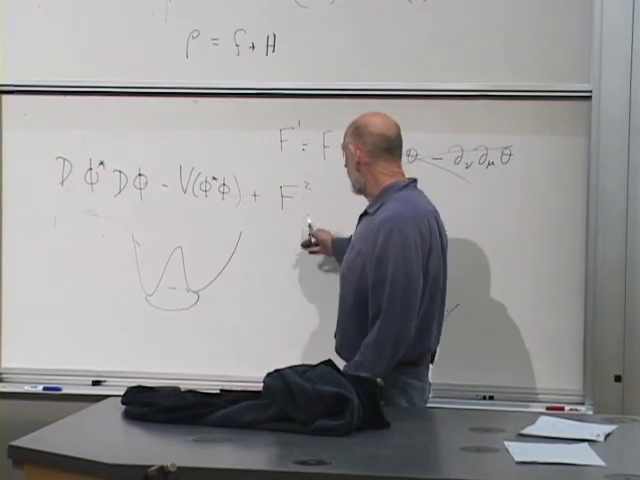
\includegraphics[width=0.76\textwidth]{lecture_08_figure_05.png}
\caption{La pizarra muestra el obstáculo: bajo una transformación gauge, \(A_\mu A^\mu\) se convierte en un cuadrado que contiene \(\partial_\mu\theta\), por lo que un término de masa desnudo para el vector no es invariante.}
\lectureframe{01:07:30}
\label{fig:l08-bare-mass-board}
\end{figure}

\section{El mecanismo de Higgs}

\subsection{La derivada covariante produce la masa}

Volvamos al potencial roto y usemos la parametrización con normalización canónica
\begin{equation}
  \phi(x)=\frac{f+h(x)}{\sqrt2}
  e^{i\pi(x)/f}.
\end{equation}
Su derivada covariante es
\begin{equation}
  D_\mu\phi
  =
  \frac{e^{i\pi/f}}{\sqrt2}
  \left[
    \partial_\mu h
    +i(f+h)
      \left(\frac{\partial_\mu\pi}{f}+gA_\mu\right)
  \right].
  \label{eq:l08-covariant-polar}
\end{equation}
Por consiguiente,
\begin{equation}
\begin{aligned}
  (D_\mu\phi)^*D^\mu\phi
  ={}&
  \frac12(\partial_\mu h)^2
  \\
  &+\frac12(f+h)^2
    \left(\frac{\partial_\mu\pi}{f}+gA_\mu\right)
  \\
  &\hspace{4.2em}\times
    \left(\frac{\partial^\mu\pi}{f}+gA^\mu\right).
\end{aligned}
  \label{eq:l08-higgs-kinetic}
\end{equation}

El término decisivo aparece antes de elegir ningún gauge:
\begin{equation}
  \frac12g^2f^2 A_\mu A^\mu.
  \label{eq:l08-vector-mass-term}
\end{equation}
Al compararlo con la forma de Proca \(\frac12m_A^2A_\mu A^\mu\), encontramos
\begin{equation}
  \boxed{m_A=g f}.
  \label{eq:l08-vector-mass}
\end{equation}
El mismo desarrollo también produce interacciones \(g^2fh A_\mu A^\mu\) y \(\frac12g^2h^2A_\mu A^\mu\). Por tanto, la masa del vector no es una violación arbitraria de la simetría gauge. Proviene de un término cinético escalar invariante gauge evaluado en una fase con magnitud de equilibrio \(f\) distinta de cero.

\begin{figure}[htbp]
\centering
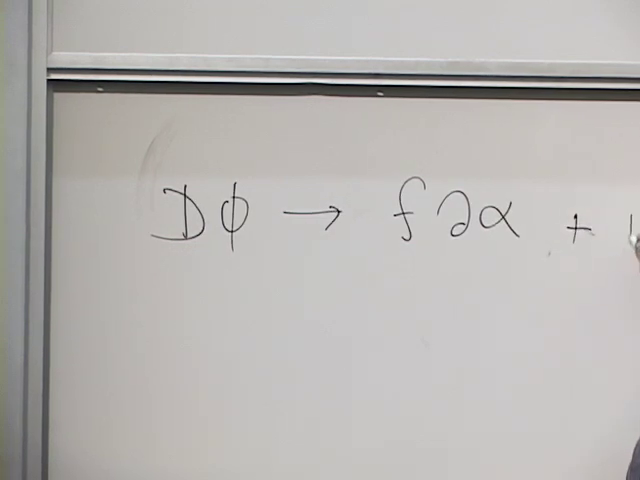
\includegraphics[width=0.78\textwidth]{lecture_08_figure_06.png}
\caption{La pizarra separa la contribución \(f^2A^2\) contenida en \((D\phi)^*(D\phi)\). Los factores numéricos dependen de cómo se normalicen el campo escalar y el acoplamiento gauge; con las ecs.~\eqref{eq:l08-canonical-polar} y \eqref{eq:l08-covariant-convention}, el resultado es \(m_A=gf\).}
\lectureframe{01:10:10}
\label{fig:l08-generated-mass-board}
\end{figure}

La clase incorpora \(g\) y varios factores de \(\sqrt2\) a la notación de la pizarra; por eso, al identificar la masa, alterna brevemente entre \(f\), \(2f\) y \(\sqrt2f\). Esos factores no tienen un significado invariante mientras no se especifiquen las normalizaciones cinética y del potencial. El resultado robusto es \(m_A\propto gf\); la ec.~\eqref{eq:l08-vector-mass} da el factor correspondiente a la convención usada aquí.

\subsection{La fase queda absorbida}

Bajo una transformación gauge, la variable de fase cambia según
\begin{equation}
  \pi'(x)=\pi(x)+f\,\theta(x).
\end{equation}
Elijamos
\begin{equation}
  \theta(x)=-\frac{\pi(x)}{f}.
  \label{eq:l08-unitary-gauge-choice}
\end{equation}
Entonces \(\pi'=0\). Este es el gauge unitario, en el que \begin{equation}
  \phi'(x)=\frac{f+h(x)}{\sqrt2}
\end{equation} es real, y la ec.~\eqref{eq:l08-higgs-kinetic} se reduce a
\begin{equation}
  (D_\mu\phi')^*D^\mu\phi'
  =
  \frac12(\partial_\mu h)^2
  +\frac12g^2(f+h)^2A_\mu'A^{\prime\mu}.
  \label{eq:l08-unitary-gauge-lagrangian}
\end{equation}
El campo de Goldstone angular ha desaparecido de la lista de variables independientes, mientras que la masa del vector permanece.

La clase muestra primero este resultado en el límite de baja energía \(\rho=f\), donde
\begin{align}
  \phi&=f e^{i\alpha},
  \notag\\
  D_\mu\phi
  &=if e^{i\alpha}
    \left(\partial_\mu\alpha+gA_\mu\right),
  \notag\\
  (D_\mu\phi)^*
  &=-if e^{-i\alpha}
    \left(\partial_\mu\alpha+gA_\mu\right).
  \label{eq:l08-frozen-radius}
\end{align}
Su producto es
\begin{equation}
  f^2
  \left(\partial_\mu\alpha+gA_\mu\right)
  \left(\partial^\mu\alpha+gA^\mu\right).
\end{equation}
La elección \(\theta=-\alpha\) deja \(g^2f^2A_\mu'A^{\prime\mu}\).

\begin{figure}[htbp]
\centering
\includegraphics[width=0.82\textwidth]{lecture_08_figure_07.png}
\caption{La pizarra muestra el desarrollo completo con radio fijo: las derivadas covariantes contienen conjuntamente la derivada de la fase y el potencial vector. A continuación, la clase elige \(\theta=-\alpha\), elimina la fase y deja el término de masa del vector.}
\lectureframe{01:16:20}
\label{fig:l08-frozen-radius-board}
\end{figure}

\begin{classroomqa}
\audiencequestion{¿Se puede reescribir todo el lagrangiano en variables que hagan explícita la desaparición del modo angular?
\lecturetimestamp{01:13:49}}
\lecturerresponse{Sí. En coordenadas polares, la fase solo aparece en la combinación invariante gauge \(\partial_\mu\alpha+gA_\mu\). Una transformación gauge con \(\theta=-\alpha\) fija la fase en cero en todos los puntos donde este gauge esté bien definido. El término cinético escalar se convierte entonces en un término de masa para el vector, mientras que el término invariante gauge del tensor de campo no cambia.}
\end{classroomqa}

\begin{classroomqa}
\audiencequestion{¿Son indistinguibles las oscilaciones de \(\alpha\) y las oscilaciones gauge?\lecturetimestamp{01:18:02}}
\lecturerresponse{En la teoría gauge, un cambio puro de \(\alpha\) compensado por el cambio correspondiente de \(A_\mu\) es una redescripción gauge, no una onda física distinta. La cantidad invariante es \(\partial_\mu\alpha+gA_\mu\). El modo físico que estaba representado por el campo global de Goldstone reaparece como la polarización longitudinal del vector masivo.}
\end{classroomqa}

Es habitual decir que una simetría gauge local se rompe espontáneamente. Esta expresión es útil en términos operativos: después de elegir un gauge, el campo escalar tiene un valor de vacío distinto de cero y el espectro contiene un vector masivo. Sin embargo, en sentido estricto, las transformaciones gauge relacionan descripciones redundantes, no estados físicos distintos.
\editorialnote{La redundancia gauge local no se rompe en el mismo sentido invariante gauge que una simetría global. La formulación precisa es que la teoría está en una fase de Higgs. La teoría de perturbaciones fijada en un gauge describe esa fase mediante un valor esperado escalar distinto de cero y el espectro resultante de vectores masivos.}

\section{Adónde fue el grado de libertad de Goldstone}

Nada físico puede desaparecer simplemente porque hayamos cambiado de variables. Contemos los grados de libertad antes y después de entrar en la fase de Higgs.

Antes:
\begin{equation}
  \underbrace{2}_{\text{massless vector}}
  +
  \underbrace{2}_{\text{complex scalar}}
  =4.
\end{equation}
Un vector sin masa tiene dos polarizaciones transversales. El escalar complejo tiene dos componentes reales: una radial y otra angular.

Después:
\begin{equation}
  \underbrace{3}_{\text{massive vector}}
  +
  \underbrace{1}_{\text{radial Higgs}}
  =4.
  \label{eq:l08-degree-count}
\end{equation}
Un vector masivo puede ponerse en reposo. En su sistema de reposo no hay ninguna dirección espacial privilegiada, así que debe tener tres estados de polarización. Cuando se mueve, dos son transversales y uno es longitudinal. El modo de Goldstone se ha convertido en esa polarización longitudinal.

\begin{figure}[htbp]
\centering
\begin{adjustbox}{max width=\linewidth}
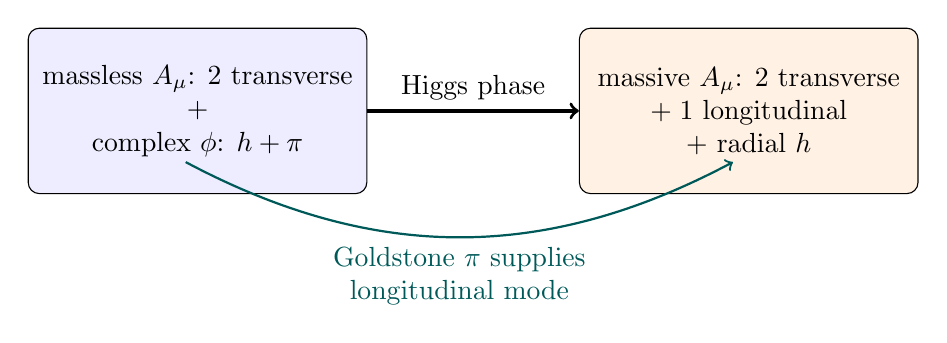
\begin{tikzpicture}[x=1cm,y=1cm]
  \node[draw,rounded corners,fill=blue!7,minimum width=4.3cm,
        minimum height=2.1cm,align=center] (before) at (0,0)
    {massless \(A_\mu\): \(2\) transverse\\
     \(+\)\\
     complex \(\phi\): \(h+\pi\)};
  \node[draw,rounded corners,fill=orange!10,minimum width=4.3cm,
        minimum height=2.1cm,align=center] (after) at (7,0)
    {massive \(A_\mu\): \(2\) transverse\\
     \(+\;1\) longitudinal\\
     \(+\) radial \(h\)};
  \draw[->,very thick] (before) -- node[above]{Higgs phase} (after);
  \draw[->,teal!70!black,thick]
    (-0.15,-0.65) to[bend right=28]
    node[below,align=center]{Goldstone \(\pi\) supplies\\longitudinal mode}
    (6.8,-0.65);
\end{tikzpicture}
\end{adjustbox}
\caption{El mecanismo de Higgs reorganiza los grados de libertad físicos, no los destruye.}
\label{fig:l08-degree-rearrangement}
\end{figure}

\begin{classroomqa}
\audiencequestion{¿Cómo puede desaparecer el grado de libertad angular sin violar el recuento de grados de libertad?\lecturetimestamp{01:19:13}}
\lecturerresponse{No desaparece físicamente. Un vector sin masa tiene dos helicidades porque no se puede poner en reposo. Un vector masivo tiene tres polarizaciones, incluida una longitudinal. El modo de Goldstone se convierte en esa tercera polarización, de modo que el número total de grados de libertad no cambia.}
\end{classroomqa}

La clase propone una prueba cinemática útil. Imaginemos una partícula vectorial masiva, reduzcamos su velocidad hasta detenerla y acelerémosla en una dirección nueva. Una polarización que era transversal respecto del movimiento inicial puede volverse longitudinal respecto del nuevo movimiento. Del mismo modo, si una partícula masiva con polarización circular pasa por el reposo y se envía en la dirección opuesta, se invierte su etiqueta de helicidad. No se puede hacer este experimento con una partícula estrictamente sin masa, porque ningún sistema inercial puede ponerla en reposo. Por tanto, sus dos helicidades constituyen un espectro físico coherente.

\section{La analogía superconductora}

En un superconductor convencional, los electrones forman pares de Cooper. Cada par es un bosón con carga eléctrica \(2e\), y el condensado se describe mediante un parámetro de orden complejo cargado. Cuando su magnitud es distinta de cero, la combinación de su fase y el potencial vector electromagnético produce el mecanismo de Anderson--Higgs. Los campos magnéticos estáticos decaen a lo largo de la profundidad de penetración de London, en vez de extenderse libremente por el interior del material. En este sentido preciso y dependiente del medio, el fotón se comporta como si hubiera adquirido masa.

Este ejemplo también aclara la distinción inicial. El campo electromagnético no se convierte de manera permanente en otra partícula elemental. La ley de propagación masiva corresponde al estado colectivo dentro del material; fuera de él, el fotón del vacío sigue sin tener masa.

\section{Qué se ha establecido}

Ahora podemos condensar el argumento sin perder su lógica:
\begin{enumerate}
  \item Una simetría continua global rota tiene una dirección angular plana y, por tanto, un modo de Goldstone sin masa.
  \item La invariancia local de fase requiere un potencial gauge y reemplaza \(\partial_\mu\) por \(D_\mu\).
  \item Una masa desnuda \(A_\mu A^\mu\) viola la ley de transformación local.
  \item Cuando el escalar cargado tiene una magnitud de equilibrio \(f\) distinta de cero, el término invariante gauge \(|D_\mu\phi|^2\) contiene \(\frac12g^2f^2A_\mu A^\mu\).
  \item El modo de fase puede eliminarse mediante una elección de gauge, y su grado de libertad físico se convierte en la polarización longitudinal del vector masivo.
  \item La excitación radial de Higgs permanece; su masa viene determinada por la curvatura del potencial escalar.
\end{enumerate}

La siguiente tarea es dar masa a los fermiones. Los electrones y los quarks no pueden emplear directamente el mecanismo vectorial; sus acoplamientos con el Higgs son interacciones de Yukawa. Cuando el escalar se estabiliza en \(f\), esas interacciones se convierten en términos de masa fermiónica.

La afirmación general de que las partículas conocidas serían sin masa sin la ruptura de simetría electrodébil requiere una última precisión. Las masas de los quarks elementales y los leptones cargados, así como las de \(W\) y \(Z\), sí se anulan junto con el valor esperado del Higgs. Sin embargo, la mayor parte de la masa del protón y del neutrón surge dinámicamente del confinamiento de la QCD y de la energía del campo fuerte, y no de las masas de los quarks debidas al Higgs. Esta distinción no altera el mecanismo de Higgs derivado aquí; delimita con precisión su ámbito de aplicación.
